\documentclass[12pt,a4paper]{article}
\usepackage[utf8x]{inputenc}
\usepackage[pdftex]{graphicx}
\PrerenderUnicode{äöüÄÖÜß}
\usepackage[ngerman]{babel}
\usepackage{enumitem}
\usepackage{amsmath}
\usepackage{color}
\usepackage[paper=a4paper,left=15mm,right=15mm,top=35mm,bottom=25mm]{geometry}
\usepackage{enumitem}
\setitemize{noitemsep}

\usepackage{titling}
\setlength{\droptitle}{-4cm}

\title{Ausarbeitung WebTech II}
\author{N. Henczi, B. Kleinhückelkoten, D. Kühn, D. Mues, D. Wirkner}
\date{30.4.2013}
\begin{document}	
\maketitle
\thispagestyle{empty}
\pagestyle{empty}

\newcommand{\TODO}[1]{\colorbox{red}{TODO: #1}}
	
\section{Einführende Phase}
In der Planung des Projekts wurden hauptsächlich drei Aspekte der Applikation diskutiert. Dies waren zunächst die \textbf{Technologien} welche die Arbeit in der Gruppe vereinfachen sollten, dann die \textbf{technischen Aspekte} und Entscheidungen, wie das Backend umgesetzt werden sollte und mit der deutlich meisten Euphorie \textbf{Aufbau und Aussehen} des Projekts.

\subsection{Eingesetzte Technologien}
Wir entschieden uns, in unserem Projekt die in der Vorlesung vorgestellten Technologien zu benutzen. Dies beinhaltet:

\begin{itemize}
\item \textit{Maven} als Buildprogramm, da es sehr einfach zu nutzen ist und gleichzeitig übersichtlich und komfortabel nutzbar ist
\item \textit{Jetty} als Server, da er mit Maven bereits mitgeliefert ist und in seinem Umfang unseren Ansprüchen vollkommen genügt
\item \textit{Hibernate} als Datenbank Schnittstelle, \TODO{warum haben wir Hibernate genommen?}
\end{itemize}

Die Kommunikation wurde dadurch, dass wir uns ein- bis zweimal jede Woche trafen auf Mailverkehr beschränkt. Das genügte, da wir von vornherein planten dass jeder seinen Aufgabenbereich kennen sollte und am Schluss die verbleibenden Aufgaben frühzeitig verteilt werden sollten. So hatten wir die Möglichkeit, alle Mitglieder zu erreichen um im Vorfeld Dinge oder Probleme anzusprechen und konnten diese dann auf den Treffen klären. \\

Um die Koordination in der Gruppe zu ermöglichen benutzten wir zusätzlich ein Versionskontrollsystem. Wir entschieden uns für \textit{GIT}, da es hier über GitHub (www.github.com) sehr einfach möglich war ein Repository anzulegen.

Da nur zwei Mitglieder mit GIT vertraut waren und auch nicht alle die Vorlesung in der Maven behandelt wurde besucht hatten, nutzte unsere Gruppe ein paar der ersten Termine zum Kennenlernen und Erklären von GIT und Maven.

\subsection{Entscheidungen in der Implementierung}
Bevor wir uns der Implementierung widmen konnten empfanden wir es als nützlich die Terminologie zu klären. Es war gemeinsamer Konsens, dass wir User haben würden, die Shouts verfassen.

Ein User $U_A$, der einem User $U_B$ ermöglichen möchte seine Nachrichten $M_{A0} \dotsc M_{An}$ einzusehen, kann $U_B$ einen \textbf{Invite} schicken. Nimmt $U_B$ diese Einladung an, ist $U_B$ ein \textbf{Fan} von $U_A$, gleichzeitig ist $U_A$ ein \textbf{Idol} von $U_B$. \\

Wir waren uns einig, dass es für unser Projekt nur diese zwei Model-Classes geben würde, \verb+Message+ (statt Shout, da Message technischer und weniger speziell ist) und \verb+User+. Welche Attribute diese Klassen haben sollten, wurde allerdings von unserer anfänglichen Idee nochmal leicht abgewandelt. 

Unser Plan war zu Beginn, dass ein User nur zwei Listen von Usern haben sollte, nämlich die Idols und die, die einen Invite geschickt bekamen. Die Logik hätte dann einen Umweg über den jeweils anderen User und dessen Idol-Liste machen müssen, was aber doppeltes Eintragen von User-Relationen verhindert hätte.

Durch das Konzept der inversen Abhängigkeit \TODO{ist es die inverse Abhängigkeit?} kann man diesen Vorteil aber beibehalten und dennoch den Komfort ermöglichen, bidirektional auf die Idols und Fans zugreifen zu können.

\subsection{Aufbau und Aussehen}
Damit wir mit dem Projekt beginnen konnten, mussten wir natürlich zu Beginn festlegen, wie es aussehen sollte. Dazu gehörte zunächst der Aufbau der Applikation, also die Unterteilung in Pages und Components. Zu den letztendlichen Entscheidungen, wie und warum wir die jetzt eingesetzte Variante gewählt haben, siehe \TODO{section von Nico}.

Wir gingen diese Aufgabe an, indem wir mit Inkscape ein SVG erstellten, das abstrakt den Aufbau der verschiedenen Seiten darstellte. Da diese abstrakten Darstellungen auch im SVG File aus gruppierten Komponenten bestanden, konnten wir diese sehr leicht verschieben, verändern und von unserem zunächst vorgestellten Modell auf eine Lösung mit sehr viel weniger redundanten Pages und vielen gemeinsam nutzbaren Components kommen.

\begin{figure}[h!]
\begin{center}
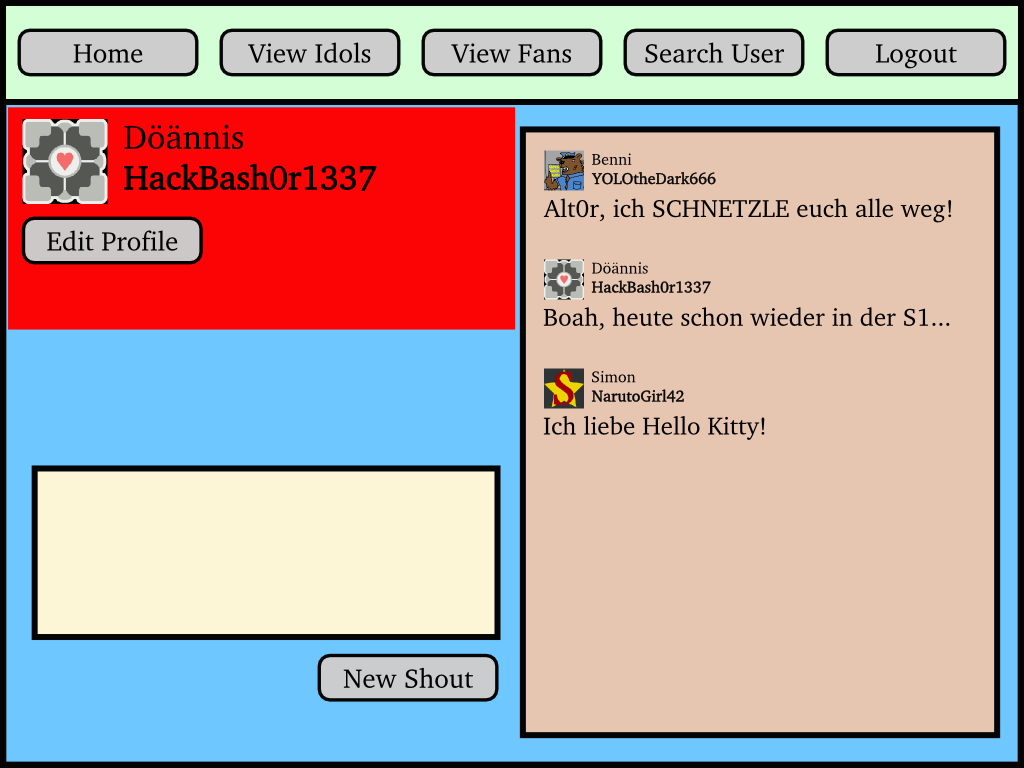
\includegraphics[width=0.9\textwidth]{entwurf.png}
\caption{Die erste Version der Ansicht zum betrachten des eigenen Profils}
\end{center}
\end{figure}


\subsection{Besondere Features und Name des Projekts}
Um das Projekt über die grundlegenen Anforderungen hinaus zu erweitern, haben wir einige Ideen für Features gesammelt, die mit realisiert werden könnten um ShoutCrowd -- wie unser Projekt genannt wurde -- noch cooler zu machen.

Der Name ShoutCrowd kam im Umfeld eines Metal-basierten Themes zustande. Eine unserer ersten Ideen war es, viele verschiedene Themes anzubieten, die der User selbst auch um eigene Themes hätte erweitern können. So wären die \verb+.properties+-Files für jedes Theme unterschiedlich und der ``Verfasse Nachricht''-Button könnte im Metal Theme ``Shout something awesome'' betitelt sein, im Gentlemen Society Theme ``Tell your fine chaps'' oder im Pirate Theme ``Name yer demand!''. An manchen Stellen wurden die besten dieser Ideen in das letztendliche Design der Seite übernommen. \\

Zudem wirkte die Seite in unseren vorgefertigten Skizzen ein wenig leer, wenn nur die Nachrichtentexte und die Namen der Verfasser angezeigt worden wären. Darum gaben wir jedem User noch die Möglichkeit, einen Avatar hochzuladen und einen persönlichen, änderbaren Nickname einzutragen. Das minutengenaue Datum der Nachricht wird ebenfalls mit angezeigt.


\end{document}